% ============================================================
% PORYGON — Upgraded Beamer Presentation (29 slides)
% pdflatex-compatible; no pgfplots dependency
% ============================================================
\documentclass[aspectratio=169,10pt]{beamer}
\usepackage[utf8]{inputenc}
\usepackage[T1]{fontenc}
\usepackage{helvet}
\renewcommand{\familydefault}{\sfdefault}
\usepackage{xcolor,booktabs,graphicx,tabularx,amsmath,amssymb,tikz}
\usepackage{array,multicol}
\usetikzlibrary{arrows.meta,positioning,calc,shapes.geometric,decorations.pathreplacing}
\graphicspath{{images/}{./}}

% ── Colour palette ──────────────────────────────────────────
\definecolor{amritaMaroon}{HTML}{A4123F}
\definecolor{lightmaroon}{HTML}{F7EAF0}
\definecolor{darkgray}{HTML}{444444}
\definecolor{lightgray}{HTML}{EEEEEE}
\definecolor{midgray}{HTML}{BBBBBB}
\colorlet{lightMaroon}{lightmaroon}
\definecolor{podFace}{HTML}{9FC7B8}
\definecolor{podTop}{HTML}{C9E4DA}
\definecolor{podSide}{HTML}{E0965C}

% ── Theme ───────────────────────────────────────────────────
\usetheme{Madrid}
\usecolortheme[named=amritaMaroon]{structure}
\setbeamertemplate{navigation symbols}{}
\setbeamertemplate{footline}[frame number]
\setbeamertemplate{itemize item}{\color{amritaMaroon}$\blacktriangleright$}

% ── Metadata ────────────────────────────────────────────────
\title[PORYGON]{PORYGON: An Image-Scoped Statistical and Rule-Based Framework\\for Container Runtime Behavioural Analysis}
\author{Ashin Varghese \and Anurup R Krishnan \and Krishnan S \and Madhav Sreejith}
\institute{Team 75 \\ 23CSE498 -- Project Phase II (External Review) \\ Guide: Dr Abirami K, Assistant Professor, Department of CSE}
\date{Amrita Vishwa Vidyapeetham, Coimbatore}

% ── Convenience TikZ styles (global) ────────────────────────
\tikzset{
  pbox/.style={draw=amritaMaroon, fill=lightmaroon, thick,
               minimum width=#1, minimum height=0.75cm, align=center,
               font=\bfseries\scriptsize},
  pbox/.default=2.4cm,
  gbox/.style={draw=darkgray!60, fill=lightgray, thick,
               minimum width=#1, minimum height=0.75cm, align=center,
               font=\scriptsize},
  gbox/.default=2.4cm,
  wbox/.style={draw=amritaMaroon, fill=white, thick,
               minimum width=#1, minimum height=0.75cm, align=center,
               font=\scriptsize},
  wbox/.default=2.4cm,
  mbox/.style={draw=amritaMaroon, fill=amritaMaroon, text=white, thick,
               minimum width=#1, minimum height=0.75cm, align=center,
               font=\bfseries\scriptsize},
  mbox/.default=2.4cm,
  arr/.style={-{Latex[length=2.5mm]}, thick, draw=black!75},
  darr/.style={-{Latex[length=2mm]}, dashed, thick, draw=amritaMaroon},
}

\begin{document}

% ===========================================================
% SLIDE 1 — Title (unchanged)
% ===========================================================
\begin{frame}[plain]\centering\vspace{0.2cm}
{\small\color{amritaMaroon}\bfseries TYPE 1 -- RESEARCH-BASED PROJECT}\\[0.45cm]
{\LARGE\bfseries\color{amritaMaroon}PORYGON}\\[0.2cm]
{\large An Image-Scoped Statistical and Rule-Based Framework for Container Runtime Behavioural Analysis}\\[0.45cm]
\begin{tabular}{|c|c|l|}\hline\textbf{S.No.}&\textbf{Register Number}&\textbf{Student Name}\\\hline
1&CB.SC.U4CSE23504&Ashin Varghese\\\hline
2&CB.SC.U4CSE23559&Anurup R Krishnan\\\hline
3&CB.SC.U4CSE23628&Krishnan S\\\hline
4&CB.SC.U4CSE23661&Madhav Sreejith\\\hline\end{tabular}\\[0.3cm]
\textbf{Guide: Dr Abirami K} -- Assistant Professor, Department of CSE\\[0.15cm]
\small 23CSE498 -- Project Phase II \quad|\quad Team 75\\Amrita Vishwa Vidyapeetham, Coimbatore
\end{frame}

% ===========================================================
% SLIDE 2 — Guide Review & Submission Approval
% ===========================================================
\begin{frame}{Guide Review \& Submission Approval}
\framesubtitle{Mandatory guide approval evidence --- 23CSE498 · Team 75}
\centering\vfill

\begin{tikzpicture}
  \node[draw=amritaMaroon, fill=lightmaroon, very thick,
        minimum width=11cm, minimum height=5cm, align=center,
        inner sep=0.4cm] (box) {
    {\large\bfseries\color{amritaMaroon}Guide Approval Evidence}\\[0.35cm]
    {\normalsize Insert a readable screenshot of Dr Abirami K's}\\
    {\normalsize approval email or signed acknowledgement here.}\\[0.4cm]
    {\small\color{darkgray}Replace this placeholder before submission.}
  };
  \draw[amritaMaroon, very thick] (box.north west) -- ++(0.4,0);
  \draw[amritaMaroon, very thick] (box.north west) -- ++(0,-0.4);
  \draw[amritaMaroon, very thick] (box.south east) -- ++(-0.4,0);
  \draw[amritaMaroon, very thick] (box.south east) -- ++(0,0.4);
\end{tikzpicture}
\vfill
\end{frame}

% ===========================================================
% SLIDE 3 — Problem Definition & Research Motivation
% ===========================================================
\section{Problem and Motivation}
\begin{frame}{1. Problem Definition \& Research Motivation}
\footnotesize

\begin{columns}[T,onlytextwidth]
\column{0.52\textwidth}
\begin{block}{Problem Statement}
\begin{itemize}
  \item \textbf{Core Problem:} Shared baselines mix unlike workloads, misclassifying image-specific process activity.
  \item \textbf{Domain Context:} Container images exhibit distinct runtime behaviour requiring workload-specific monitoring.
\end{itemize}
\end{block}
\vspace{0.15cm}
\begin{block}{Research Objectives}
\begin{itemize}
  \item \textbf{Obj. 1:} Build image-specific baselines using immutable OCI digests.
  \item \textbf{Obj. 2:} Hybrid detection via JSD distance, novelty, numerical deviation, and deterministic rules.
  \item \textbf{Obj. 3:} Measure profile-scope effect on identical workload runs.
\end{itemize}
\end{block}

\column{0.46\textwidth}
\begin{block}{Conventional vs.\ Image-Scoped Monitoring}
\renewcommand{\arraystretch}{1.25}
\begin{tabularx}{\linewidth}{>{\bfseries}p{1.9cm} X}
\toprule
Aspect & Comparison \\\midrule
Baseline scope & Global / tag-based vs.\ digest-pinned \\
Workload mixing & All containers vs.\ same-image only \\
Identity drift & Tag can change vs.\ digest is immutable \\
False-alarm risk & Higher (mixed) vs.\ Lower (scoped) \\
Evidence & Score only vs.\ Score + rule provenance \\
\bottomrule
\end{tabularx}
\end{block}
\end{columns}
\end{frame}

% ===========================================================
% SLIDE 4 — Research Gap & Objectives
% ===========================================================
\begin{frame}{2. Research Gap \& Objectives}
\small

\begin{block}{Existing Approaches \& Their Limits}
\begin{itemize}
  \item System-call bag-of-words models lose temporal sequence context.
  \item eBPF / Falco rule-only approaches produce binary verdicts with no ranked score.
  \item ML models require labelled attack data and lack interpretable evidence per finding.
  \item \textbf{Shared gap:} None bind a behavioural model to an \emph{immutable image identity}; tag-based grouping silently merges different image versions.
\end{itemize}
\end{block}

\vspace{0.2cm}

\begin{columns}[T,onlytextwidth]
\column{0.48\textwidth}
\begin{alertblock}{Identified Gap}
No prior work combines:\\
(a) digest-scoped statistical profiling,\\
(b) hybrid JSD + rule detection, and\\
(c) human-approved containment\\
in a single reviewable incident workflow.
\end{alertblock}

\column{0.48\textwidth}
\begin{block}{Our Objectives}
\begin{enumerate}\setlength{\itemsep}{3pt}
  \item Digest-scoped versioned profiles
  \item Bounded JSD + novelty + numerical deviation
  \item Seven deterministic rules with provenance
  \item Approval-gated pause / stop response
  \item Reproducible pilot evaluation design
\end{enumerate}
\end{block}
\end{columns}
\end{frame}

% ===========================================================
% SLIDE 5 — Threat Model & Attack Surface
% ===========================================================
\begin{frame}{3. Threat Model \& Attack Surface}
\centering
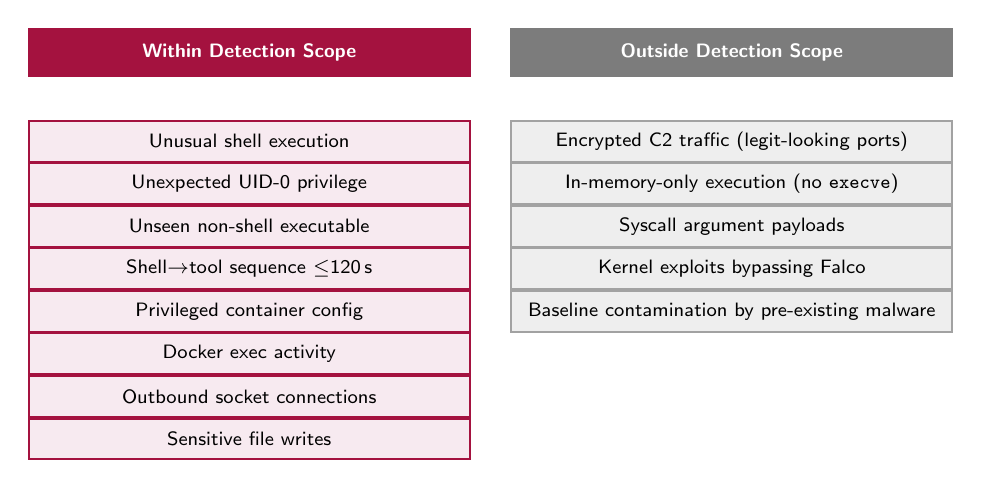
\begin{tikzpicture}[font=\scriptsize, node distance=0.28cm]

  % ── Left column header ──
  \node[draw=amritaMaroon, fill=amritaMaroon, text=white, thick,
        minimum width=5.6cm, minimum height=0.6cm, align=center,
        font=\bfseries\scriptsize] (lh) at (0,0)
        {Within Detection Scope};

  % ── Left items ──
  \foreach \txt/\idx in {%
    {Unusual shell execution}/1,
    {Unexpected UID-0 privilege}/2,
    {Unseen non-shell executable}/3,
    {Shell$\to$tool sequence $\leq$120\,s}/4,
    {Privileged container config}/5,
    {Docker exec activity}/6,
    {Outbound socket connections}/7,
    {Sensitive file writes}/8%
  }{
    \node[draw=amritaMaroon, fill=lightmaroon, thick,
          minimum width=5.6cm, minimum height=0.52cm, align=center,
          below=0.0cm of lh, yshift={-\idx*0.54cm}]
          (li\idx) {\txt};
  }

  % ── Right column header ──
  \node[draw=darkgray!70, fill=darkgray!70, text=white, thick,
        minimum width=5.6cm, minimum height=0.6cm, align=center,
        font=\bfseries\scriptsize, right=0.5cm of lh] (rh)
        {Outside Detection Scope};

  % ── Right items ──
  \foreach \txt/\idx in {%
    {Encrypted C2 traffic (legit-looking ports)}/1,
    {In-memory-only execution (no \texttt{execve})}/2,
    {Syscall argument payloads}/3,
    {Kernel exploits bypassing Falco}/4,
    {Baseline contamination by pre-existing malware}/5%
  }{
    \node[draw=darkgray!50, fill=lightgray, thick,
          minimum width=5.6cm, minimum height=0.52cm, align=center,
          below=0.0cm of rh, yshift={-\idx*0.54cm}]
          (ri\idx) {\txt};
  }

\end{tikzpicture}
\end{frame}

% ===========================================================
% SLIDE 6 — System Architecture
% ===========================================================
\begin{frame}{4. System Architecture}
\centering
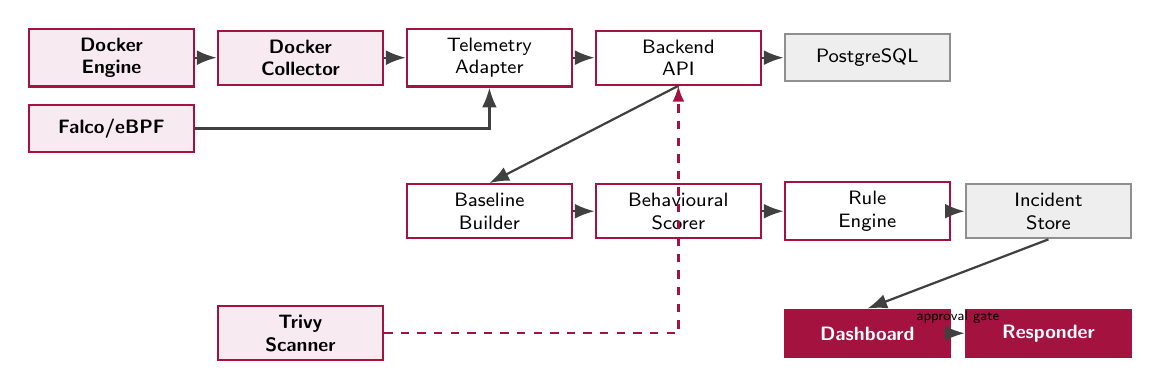
\begin{tikzpicture}[font=\scriptsize, node distance=0.18cm and 0.22cm,
    cnode/.style={draw=amritaMaroon, fill=lightmaroon, thick,
                  minimum width=2.1cm, minimum height=0.6cm,
                  align=center, font=\bfseries\scriptsize},
    pnode/.style={draw=amritaMaroon, fill=white, thick,
                  minimum width=2.1cm, minimum height=0.6cm,
                  align=center, font=\scriptsize},
    snode/.style={draw=darkgray!60, fill=lightgray, thick,
                  minimum width=2.1cm, minimum height=0.6cm,
                  align=center, font=\scriptsize},
    onode/.style={draw=amritaMaroon, fill=amritaMaroon, text=white, thick,
                  minimum width=2.1cm, minimum height=0.6cm,
                  align=center, font=\bfseries\scriptsize},
  ]

  % Row 1 — collection
  \node[cnode] (docker)  at (0,0)       {Docker\\Engine};
  \node[cnode] (falco)   at (0,-0.9)    {Falco/eBPF};
  \node[cnode] (coll)    at (2.4,0)     {Docker\\Collector};
  \node[pnode] (telem)   at (4.8,0)     {Telemetry\\Adapter};
  \node[pnode] (api)     at (7.2,0)     {Backend\\API};
  \node[snode] (pg)      at (9.6,0)     {PostgreSQL};

  % Row 2 — processing
  \node[pnode] (bb)      at (4.8,-1.95) {Baseline\\Builder};
  \node[pnode] (scorer)  at (7.2,-1.95) {Behavioural\\Scorer};
  \node[pnode] (rules)   at (9.6,-1.95) {Rule\\Engine};
  \node[snode] (inc)     at (11.9,-1.95){Incident\\Store};

  % Row 3 — operator + scanner
  \node[onode] (dash)    at (9.6,-3.5)  {Dashboard};
  \node[onode] (resp)    at (11.9,-3.5) {Responder};
  \node[cnode] (trivy)   at (2.4,-3.5)  {Trivy\\Scanner};

  % Arrows — collection path
  \draw[arr] (docker.east)  -- (coll.west);
  \draw[arr] (falco.east)   -| (telem.south);
  \draw[arr] (coll.east)    -- (telem.west);
  \draw[arr] (telem.east)   -- (api.west);
  \draw[arr] (api.east)     -- (pg.west);

  % Arrows — processing path
  \draw[arr] (api.south)    -- (bb.north);
  \draw[arr] (bb.east)      -- (scorer.west);
  \draw[arr] (scorer.east)  -- (rules.west);
  \draw[arr] (rules.east)   -- (inc.west);

  % Arrows — operator path
  \draw[arr] (inc.south)    -- (dash.north);
  \draw[arr] (dash.east)    -- (resp.west)
             node[midway, above, font=\tiny] {approval gate};

  % Arrows — scanner
  \draw[darr] (trivy.east)  -| (api.south);

\end{tikzpicture}

\vspace{0.1cm}
{\scriptsize\color{darkgray}
\textbf{Legend:}
\tikz{\node[draw=amritaMaroon,fill=lightmaroon,minimum width=0.5cm,minimum height=0.3cm]{};}\, Collection \quad
\tikz{\node[draw=amritaMaroon,fill=white,minimum width=0.5cm,minimum height=0.3cm]{};}\, Processing \quad
\tikz{\node[draw=darkgray!60,fill=lightgray,minimum width=0.5cm,minimum height=0.3cm]{};}\, Storage \quad
\tikz{\node[draw=amritaMaroon,fill=amritaMaroon,text=white,minimum width=0.5cm,minimum height=0.3cm]{};}\, Operator-facing
}
\end{frame}

% ===========================================================
% SLIDE 7 — End-to-End Workflow (original TikZ, cleaned)
% ===========================================================
\begin{frame}{5. End-to-End Workflow}
\centering
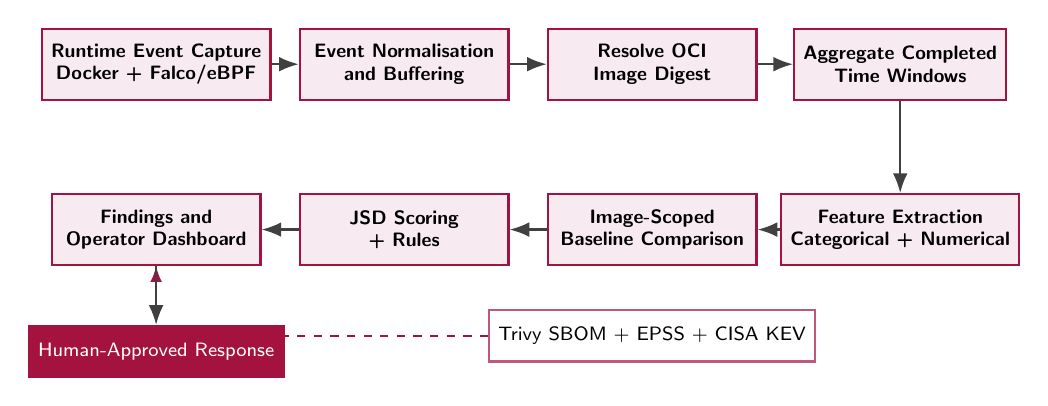
\begin{tikzpicture}[
    font=\scriptsize,
    process/.style={
        draw=amritaMaroon, fill=lightmaroon, thick,
        minimum width=2.65cm, minimum height=0.9cm,
        align=center, font=\bfseries\scriptsize},
    auxiliary/.style={
        draw=amritaMaroon!70, fill=white, thick,
        minimum width=2.5cm, minimum height=0.65cm,
        align=center, font=\scriptsize},
    flow/.style={-{Latex[length=2.5mm]}, thick, draw=black!75},
    optional/.style={-{Latex[length=2mm]}, dashed, thick, draw=amritaMaroon}
]

\node[process] (capture)   at (0,0)      {Runtime Event Capture\\Docker + Falco/eBPF};
\node[process] (normalise) at (3.15,0)   {Event Normalisation\\and Buffering};
\node[process] (identity)  at (6.3,0)    {Resolve OCI\\Image Digest};
\node[process] (window)    at (9.45,0)   {Aggregate Completed\\Time Windows};

\node[process] (features)  at (9.45,-2.1){Feature Extraction\\Categorical + Numerical};
\node[process] (baseline)  at (6.3,-2.1) {Image-Scoped\\Baseline Comparison};
\node[process] (detection) at (3.15,-2.1){JSD Scoring\\+ Rules};
\node[process] (finding)   at (0,-2.1)   {Findings and\\Operator Dashboard};

\draw[flow] (capture)   -- (normalise);
\draw[flow] (normalise) -- (identity);
\draw[flow] (identity)  -- (window);
\draw[flow] (window.south) -- (features.north);
\draw[flow] (features)  -- (baseline);
\draw[flow] (baseline)  -- (detection);
\draw[flow] (detection) -- (finding);

\node[auxiliary] (vuln) at (6.3,-3.45) {Trivy SBOM + EPSS + CISA KEV};
\draw[optional] (vuln.west) -| (finding.south);

\node[auxiliary, fill=amritaMaroon, text=white, draw=amritaMaroon]
     (response) at (0,-3.65) {Human-Approved Response};
\draw[flow] (finding.south) -- (response.north);

\end{tikzpicture}

\vspace{0.2cm}
\begin{block}{}
\scriptsize
Runtime events are collected, normalised, and associated with an immutable image digest. Completed windows are scored; evidence is retained for dashboard review. Containment requires explicit operator approval.
\end{block}
\end{frame}

% ===========================================================
% SLIDE 8 — Image-Scoped Baseline Construction
% ===========================================================
\begin{frame}[shrink=2]{6. Image-Scoped Baseline Construction}
\small

\begin{columns}[T,onlytextwidth]
\column{0.52\textwidth}
\begin{enumerate}
  \item Collect container lifecycle and process-execution events.
  \item Associate each container with its immutable OCI image digest.
  \item Group observations by digest to preserve image-specific behaviour.
  \item Aggregate observations into fixed-length time windows.
  \item Build an approved versioned profile with a training interval and support check.
  \item Compare completed runtime windows against the matching image-specific profile.
\end{enumerate}
\begin{alertblock}{Why Image Digest?}
\scriptsize An OCI tag can point to different image versions over time. An immutable digest provides a stable identity for associating runtime observations with the correct profile.
\end{alertblock}

\column{0.44\textwidth}
\begin{block}{Two Digests — Two Profiles}
\centering
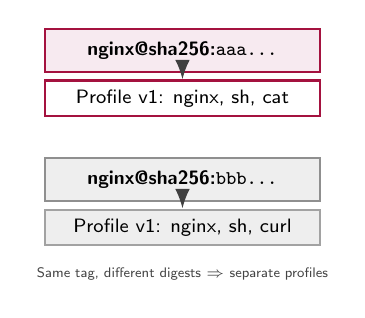
\begin{tikzpicture}[font=\scriptsize, node distance=0.2cm]
  \node[draw=amritaMaroon, fill=lightmaroon, thick,
        minimum width=3.5cm, minimum height=0.55cm, align=center,
        font=\bfseries\scriptsize] (d1)
        {nginx@sha256:\texttt{aaa\ldots}};

  \node[draw=amritaMaroon, fill=white, thick,
        minimum width=3.5cm, minimum height=0.42cm, align=center,
        below=0.08cm of d1] (p1)
        {Profile v1: nginx, sh, cat};

  \node[draw=darkgray!60, fill=lightgray, thick,
        minimum width=3.5cm, minimum height=0.55cm, align=center,
        font=\bfseries\scriptsize, below=0.5cm of p1] (d2)
        {nginx@sha256:\texttt{bbb\ldots}};

  \node[draw=darkgray!50, fill=lightgray, thick,
        minimum width=3.5cm, minimum height=0.42cm, align=center,
        below=0.08cm of d2] (p2)
        {Profile v1: nginx, sh, curl};

  \draw[arr] (d1.south) -- (p1.north);
  \draw[arr] (d2.south) -- (p2.north);

  \node[font=\tiny, below=0.15cm of p2, text=darkgray]
        {Same tag, different digests $\Rightarrow$ separate profiles};
\end{tikzpicture}
\end{block}
\end{columns}
\end{frame}

% ===========================================================
% SLIDE 9 — Feature Representation
% ===========================================================
\begin{frame}{7. Feature Representation}
\small

\begin{columns}[T,onlytextwidth]
\column{0.49\textwidth}
\begin{block}{Categorical Features}
\begin{itemize}
  \item Executable identity
  \item Parent--child process edges
  \item Process-sequence bigrams
  \item Process names
  \item User identifiers
  \item Runtime actions
  \item Command shape: subcommands, flags, argument classes, shell composition
\end{itemize}
\end{block}

\column{0.49\textwidth}
\begin{block}{Numerical Features}
\begin{itemize}
  \item Distinct processes per window
  \item Process-event rate
  \item Root-process ratio
  \item Shell-process ratio
  \item Runtime-event rate
\end{itemize}
\end{block}

\end{columns}

\vspace{0.15cm}

\begin{block}{Input Sources}
Falco/eBPF process-execution telemetry and Docker lifecycle information, normalised through the telemetry adapter.
\end{block}
\end{frame}

% ===========================================================
% SLIDE 10 — Feature Extraction Example
% ===========================================================
\begin{frame}{8. Feature Extraction Example}
\footnotesize
\begin{block}{Raw Falco \texttt{execve} Event $\rightarrow$ Feature Vector}
\centering\renewcommand{\arraystretch}{1.3}
\begin{tabularx}{0.96\textwidth}{>{\bfseries}p{2.6cm} l X}
\toprule
Field & Raw Value & Extracted Feature \\\midrule
\texttt{proc.name}      & \texttt{curl}        & executable\_token = ``curl'' \\
\texttt{proc.exepath}   & \texttt{/usr/bin/curl} & full executable path recorded \\
\texttt{proc.pname}     & \texttt{bash}        & parent\_child\_edge = ``bash$\to$curl'' \\
\texttt{user.uid}       & \texttt{0}           & user\_uid\_token = ``0'' (root) \\
\texttt{evt.time} offset & \texttt{T+45\,s}    & within 120\,s window; Rule 005 eligible \\
\midrule
\multicolumn{2}{l}{\textbf{Novelty signal}} &
  ``curl'' absent from baseline executable distribution $\Rightarrow$ novelty contribution = 1.0 \\
\multicolumn{2}{l}{\textbf{Numerical update}} &
  root\_process\_ratio increases; shell\_process\_ratio unchanged \\
\bottomrule
\end{tabularx}
\end{block}

\vspace{0.1cm}
\begin{alertblock}{}
\scriptsize Every field is treated as an observation token; absence from the approved profile vocabulary contributes directly to the novelty score $V$.
\end{alertblock}
\end{frame}

% ===========================================================
% SLIDE 11 — Jensen–Shannon Distance + bar chart
% ===========================================================
\begin{frame}{9. Jensen--Shannon Distance}
\footnotesize

\begin{columns}[T,onlytextwidth]
\column{0.44\textwidth}
\begin{block}{Definition}
\centering
\[M = \dfrac{P+Q}{2}\]
\[D_{JS}(P,Q) = \sqrt{\tfrac{1}{2}D_{KL}(P\|M) + \tfrac{1}{2}D_{KL}(Q\|M)}\]
\end{block}

\vspace{0.1cm}
\begin{itemize}\setlength{\itemsep}{3pt}
  \item \textbf{Symmetric:} $D_{JS}(P,Q)=D_{JS}(Q,P)$
  \item \textbf{Bounded:} $D_{JS}\in[0,1]$ (base-2 logs)
  \item \textbf{Finite:} handles non-overlapping support
  \item \textbf{Metric:} satisfies triangle inequality
\end{itemize}

\column{0.54\textwidth}
\begin{block}{Illustrative Distributions — $D_{JS}\approx 1.0$}
\centering
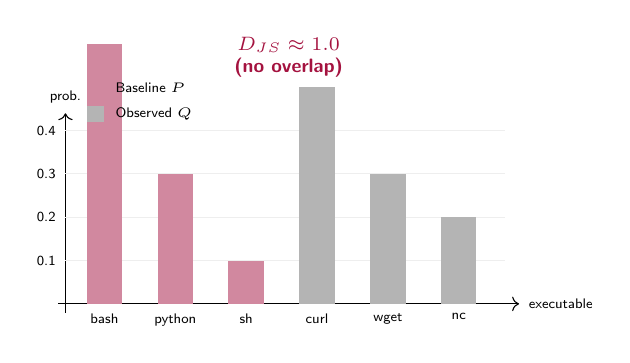
\begin{tikzpicture}[font=\tiny, xscale=0.9, yscale=1.1]
  % Axes
  \draw[->] (-0.1,0) -- (6.4,0) node[right] {executable};
  \draw[->] (0,-0.1) -- (0,2.2)  node[above] {prob.};

  % Y ticks
  \foreach \y/\lbl in {0.5/0.1, 1.0/0.2, 1.5/0.3, 2.0/0.4}{
    \draw[lightgray] (0,\y) -- (6.2,\y);
    \node[left] at (0,\y) {\lbl};
  }

  % Baseline P (blue-ish = amritaMaroon fill with 40% opacity)
  % bash=0.6, python=0.3, sh=0.1
  \fill[amritaMaroon!50] (0.3,0) rectangle ++(0.5,3.0);
  \fill[amritaMaroon!50] (1.3,0) rectangle ++(0.5,1.5);
  \fill[amritaMaroon!50] (2.3,0) rectangle ++(0.5,0.5);

  % Observed Q (gray)
  % curl=0.5, wget=0.3, nc=0.2
  \fill[darkgray!40] (3.3,0) rectangle ++(0.5,2.5);
  \fill[darkgray!40] (4.3,0) rectangle ++(0.5,1.5);
  \fill[darkgray!40] (5.3,0) rectangle ++(0.5,1.0);

  % Labels
  \node[below] at (0.55,0) {bash};
  \node[below] at (1.55,0) {python};
  \node[below] at (2.55,0) {sh};
  \node[below] at (3.55,0) {curl};
  \node[below] at (4.55,0) {wget};
  \node[below] at (5.55,0) {nc};

  % Legend
  \fill[amritaMaroon!50] (0.3,2.4) rectangle ++(0.25,0.18);
  \node[right] at (0.57,2.49) {Baseline $P$};
  \fill[darkgray!40] (0.3,2.1) rectangle ++(0.25,0.18);
  \node[right] at (0.57,2.19) {Observed $Q$};

  % DJS label
  \node[align=center, font=\scriptsize\bfseries, text=amritaMaroon]
       at (3.15,2.85) {$D_{JS}\approx 1.0$\\(no overlap)};
\end{tikzpicture}
\end{block}
\end{columns}
\end{frame}

% ===========================================================
% SLIDE 12 — Combined Scoring Model + worked example
% ===========================================================
\begin{frame}{10. Combined Score and Operating Bands}
\small

\[S=\alpha D + \beta V + \gamma N,\quad \alpha+\beta+\gamma=1\]

\begin{columns}[T,onlytextwidth]
\column{0.48\textwidth}
\begin{block}{Component Definitions}
\begin{itemize}\setlength{\itemsep}{2pt}
  \item $D$: weighted categorical distribution distance
  \item $V$: novelty of items absent from baseline
  \item $N$: scaled numerical deviation, $N\in[0,1]$
\end{itemize}
\end{block}

\vspace{0.1cm}
\begin{table}\centering\small
\begin{tabular}{ll}\toprule\textbf{Band}&\textbf{Score range}\\\midrule
Baseline-like&$S<0.25$\\Elevated&$0.25\leq S<0.50$\\High&$0.50\leq S<0.75$\\Extreme&$S\geq 0.75$\\\bottomrule\end{tabular}
\end{table}

\column{0.50\textwidth}
\begin{alertblock}{Illustrative Worked Example}
{\tiny\textit{(Illustrative values --- not from a controlled benchmark)}}\\[0.1cm]
\renewcommand{\arraystretch}{1.2}
\begin{tabular}{lll}\toprule
Component & Value & Source \\\midrule
$D$ (categorical) & 0.82 & executable family\\
$V$ (novelty) & 1.00 & curl, wget absent\\
$N$ (numerical) & 0.45 & root\_ratio $z=3.1$\\\midrule
$\alpha,\beta,\gamma$ & 0.50, 0.30, 0.20 & configured \\\midrule
\multicolumn{3}{@{}l@{}}{$\scriptstyle S = 0.50\!\times\!0.82 + 0.30\!\times\!1.0 + 0.20\!\times\!0.45$}\\
\multicolumn{3}{@{}l@{}}{$\scriptstyle\phantom{S} = 0.41 + 0.30 + 0.09 = \mathbf{0.80}$}\\
\multicolumn{3}{@{}l@{}}{\textbf{Band: Extreme}}\\
\bottomrule
\end{tabular}
\end{alertblock}
\end{columns}
\end{frame}

% ===========================================================
% SLIDE 13 — Deterministic Detection Rules
% ===========================================================
\section{Detection Rules}
\begin{frame}{11. Deterministic Rules}
\small
\vspace{0.15cm}
\begin{table}
\centering
\renewcommand{\arraystretch}{1.35}
\begin{tabularx}{0.98\textwidth}{c X c c c}
\toprule
\textbf{Rule} & \textbf{Trigger Condition} & \textbf{Incident?} & \textbf{Sev.\ Wt} & \textbf{Conf.\ Wt} \\
\midrule
001 & Completed window distance $\geq 0.50$               & No  & 0.40 & 0.50 \\
002 & Shell executable absent from baseline executed      & Yes & 0.75 & 0.70 \\
003 & UID-0 process executed; UID-0 absent from baseline  & Yes & 0.80 & 0.75 \\
004 & Previously unseen non-shell executable              & Yes & 0.70 & 0.65 \\
005 & Unseen shell $\to$ unseen non-shell, $\leq120$\,s   & Yes & 0.90 & 0.80 \\
006 & Docker exec activity during observation window      & No  & 0.50 & 0.55 \\
007 & Container reports privileged mode                   & Yes & 0.85 & 0.80 \\
\bottomrule
\end{tabularx}
\end{table}

\vspace{0.1cm}
\begin{block}{Downstream Gate}
\small
\textbf{Pause:} severity $\geq 0.70$ \emph{and} confidence $\geq 0.55$.\\
\textbf{Stop:} severity $\geq 0.90$, confidence $\geq 0.75$, \emph{and} Rule 005 or 007 matched.
\end{block}
\end{frame}

% ===========================================================
% SLIDE 14 — Human-Governed Response Policy
% ===========================================================
\begin{frame}{12. Human-Governed Response Policy}
\begin{itemize}
  \item The system records observations and generates response recommendations.
  \item Pause and stop eligibility depends on configured severity and confidence thresholds.
  \item A stop recommendation additionally requires a designated high-risk rule (005 or 007).
  \item Every disruptive action requires explicit human approval.
  \item The responder records approval metadata before pause or stop execution.
  \item Live execution is disabled by default; protected containers are never modified.
\end{itemize}
\begin{block}{Design Rationale}
The score represents behavioural difference, not a calibrated probability of attack. Human approval prevents an anomaly score alone from triggering disruptive action.
\end{block}
\end{frame}

% ===========================================================
% SLIDE 15 — SBOM and Vulnerability Enrichment
% ===========================================================
\section{Component Advisory Enrichment}
\begin{frame}{13. SBOM and Component Advisory Enrichment}
\small

\textbf{Pipeline:} Pinned Trivy 0.72.0 $\rightarrow$ CycloneDX SBOM $\rightarrow$ Advisory matching $\rightarrow$ EPSS and CISA-KEV cross-reference.

\vspace{0.15cm}

\begin{columns}[T,onlytextwidth]
\column{0.50\textwidth}
\begin{block}{Scan Results}
\renewcommand{\arraystretch}{1.3}
\begin{tabularx}{\linewidth}{X c c}
\toprule
\textbf{Image} & \textbf{Comps.} & \textbf{Findings} \\\midrule
alpine:3.20        & 15  & 0   \\
postgres:17.10-bookworm & 150 & 453 (182 CVEs) \\
\bottomrule
\end{tabularx}
\end{block}
\vspace{0.1cm}
\begin{itemize}\setlength{\itemsep}{3pt}\scriptsize
  \item 421/453 findings have live EPSS score.
  \item 0 CISA-KEV listed.
  \item All carry \texttt{exploit\_status=not\_established}.
\end{itemize}

\column{0.47\textwidth}
\begin{block}{\texttt{postgres:17.10-bookworm} Severity Split}
\centering
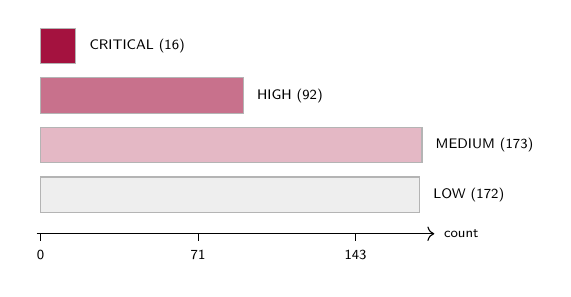
\begin{tikzpicture}[font=\tiny, xscale=1.0, yscale=0.9]
  % Horizontal bars
  % CRITICAL=16, HIGH=92, MEDIUM=173, LOW=172 (total=453)
  \def\scale{0.028}
  \foreach \sev/\cnt/\col/\y in {%
    CRITICAL/16/amritaMaroon/2.4,
    HIGH/92/amritaMaroon!60/1.7,
    MEDIUM/173/amritaMaroon!30/1.0,
    LOW/172/lightgray/0.3%
  }{
    \pgfmathsetmacro{\bw}{\cnt*\scale}
    \fill[\col, draw=darkgray!40] (0,\y) rectangle (\bw,\y+0.5);
    \node[right] at (\bw+0.05,\y+0.25) {\sev\ (\cnt)};
  }
  \draw[->] (-0.05,0) -- (5.0,0) node[right] {count};
  \foreach \x/\lbl in {0/0, 2.0/71, 4.0/143}{
    \draw (\x,0) -- (\x,-0.1) node[below] {\lbl};
  }
\end{tikzpicture}
\end{block}
\end{columns}
\end{frame}

% ===========================================================
% SLIDE 16 — Implementation Architecture (Tech Stack)
% ===========================================================
\section{Implementation and Demonstration}
\begin{frame}{14. Implementation Architecture}
\centering
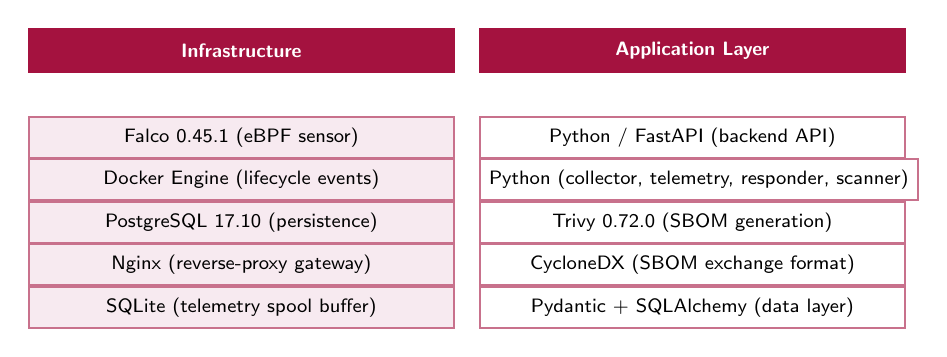
\begin{tikzpicture}[font=\scriptsize, node distance=0.2cm and 0.3cm]

  % Column headers
  \node[draw=amritaMaroon, fill=amritaMaroon, text=white, thick,
        minimum width=5.4cm, minimum height=0.55cm, align=center,
        font=\bfseries\scriptsize] (ih) at (0,0) {Infrastructure};

  \node[draw=amritaMaroon, fill=amritaMaroon, text=white, thick,
        minimum width=5.4cm, minimum height=0.55cm, align=center,
        font=\bfseries\scriptsize, right=0.3cm of ih] (ah) {Application Layer};

  % Infrastructure rows
  \foreach \txt/\idx in {%
    {Falco 0.45.1 (eBPF sensor)}/1,
    {Docker Engine (lifecycle events)}/2,
    {PostgreSQL 17.10 (persistence)}/3,
    {Nginx (reverse-proxy gateway)}/4,
    {SQLite (telemetry spool buffer)}/5%
  }{
    \node[draw=amritaMaroon!60, fill=lightmaroon, thick,
          minimum width=5.4cm, minimum height=0.52cm, align=center,
          below=0.0cm of ih, yshift={-\idx*0.54cm}] (il\idx) {\txt};
  }

  % Application rows
  \foreach \txt/\idx in {%
    {Python / FastAPI (backend API)}/1,
    {Python (collector, telemetry, responder, scanner)}/2,
    {Trivy 0.72.0 (SBOM generation)}/3,
    {CycloneDX (SBOM exchange format)}/4,
    {Pydantic + SQLAlchemy (data layer)}/5%
  }{
    \node[draw=amritaMaroon!60, fill=white, thick,
          minimum width=5.4cm, minimum height=0.52cm, align=center,
          right=0.3cm of il\idx] (al\idx) {\txt};
  }

\end{tikzpicture}
\end{frame}

% ===========================================================
% SLIDE 17 — Database & Data Flow (ER diagram)
% ===========================================================
\begin{frame}{15. Database \& Data Flow}
\centering
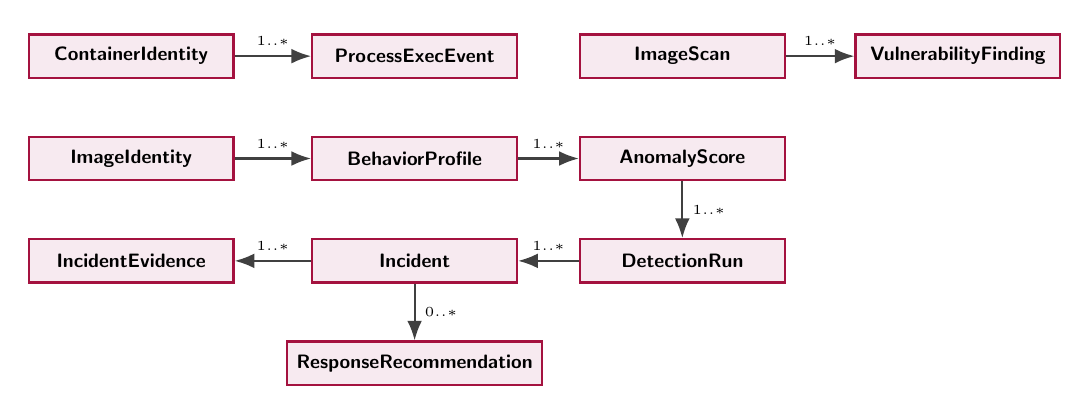
\begin{tikzpicture}[font=\scriptsize, node distance=0.5cm and 0.6cm,
  ent/.style={draw=amritaMaroon, fill=lightmaroon, thick,
              minimum width=2.6cm, minimum height=0.55cm,
              align=center, font=\bfseries\scriptsize},
  rel/.style={draw=darkgray!60, fill=lightgray, thick,
              minimum width=1.0cm, minimum height=0.42cm,
              align=center, font=\tiny},
  ]

  % Entities
  \node[ent] (ci)  at (0,0)       {ContainerIdentity};
  \node[ent] (pee) at (3.6,0)     {ProcessExecEvent};
  \node[ent] (ii)  at (0,-1.3)    {ImageIdentity};
  \node[ent] (bp)  at (3.6,-1.3)  {BehaviorProfile};
  \node[ent] (as)  at (7.0,-1.3)  {AnomalyScore};
  \node[ent] (dr)  at (7.0,-2.6)  {DetectionRun};
  \node[ent] (inc) at (3.6,-2.6)  {Incident};
  \node[ent] (ie)  at (0,-2.6)    {IncidentEvidence};
  \node[ent] (rr)  at (3.6,-3.9)  {ResponseRecommendation};
  \node[ent] (is)  at (7.0,0)     {ImageScan};
  \node[ent] (vf)  at (10.5,0)    {VulnerabilityFinding};

  % Relations
  \draw[arr] (ci.east)  -- node[above,font=\tiny]{$1..*$} (pee.west);
  \draw[arr] (ii.east)  -- node[above,font=\tiny]{$1..*$} (bp.west);
  \draw[arr] (bp.east)  -- node[above,font=\tiny]{$1..*$} (as.west);
  \draw[arr] (as.south) -- node[right,font=\tiny]{$1..*$} (dr.north);
  \draw[arr] (dr.west)  -- node[above,font=\tiny]{$1..*$} (inc.east);
  \draw[arr] (inc.west) -- node[above,font=\tiny]{$1..*$} (ie.east);
  \draw[arr] (inc.south)-- node[right,font=\tiny]{$0..*$} (rr.north);
  \draw[arr] (is.east)  -- node[above,font=\tiny]{$1..*$} (vf.west);

\end{tikzpicture}
\end{frame}

% ===========================================================
% SLIDE 18 — Attack Execution Timeline
% ===========================================================
\begin{frame}{16. Attack Execution Timeline (Shell-to-Downloader)}
\centering
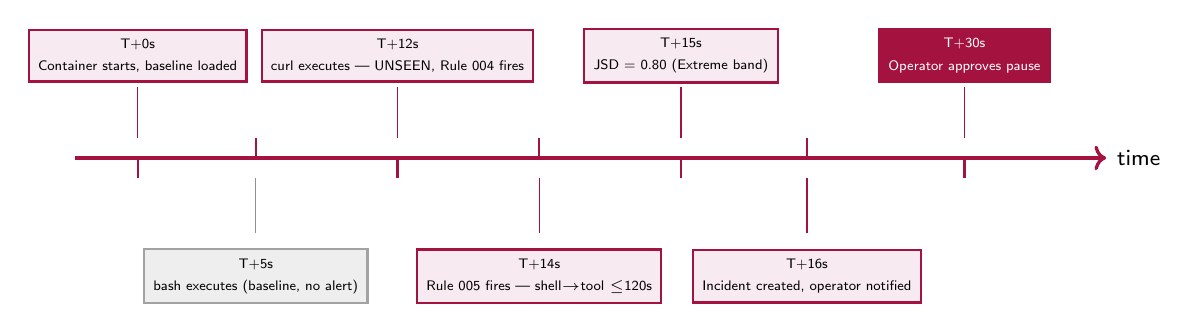
\begin{tikzpicture}[font=\scriptsize]

  % Timeline axis
  \draw[very thick, ->, draw=amritaMaroon] (-0.3,0) -- (12.8,0)
        node[right, font=\footnotesize] {time};

  % Events: (x, label above, label below)
  \def\events{%
    {0.5}/{T+0s}/{Container starts,\\baseline loaded}/%
    {2.0}/{T+5s}/{bash executes\\(baseline — no alert)}/%
    {3.8}/{T+12s}/{curl executes\\UNSEEN $\to$ Rule 004}/%
    {5.6}/{T+14s}/{Rule 005 fires\\shell$\to$tool $\leq$120s}/%
    {7.4}/{T+15s}/{JSD=0.80\\(Extreme band)}/%
    {9.0}/{T+16s}/{Incident created\\operator notified}/%
    {11.0}/{T+30s}/{Operator approves\\pause action}%
  }

  \foreach \x/\ta/\tb [count=\i] in {%
    0.5/T+0s/{Container starts, baseline loaded},
    2.0/T+5s/{bash executes (baseline, no alert)},
    3.8/T+12s/{curl executes — UNSEEN, Rule 004 fires},
    5.6/T+14s/{Rule 005 fires — shell$\to$tool $\leq$120s},
    7.4/T+15s/{JSD = 0.80 (Extreme band)},
    9.0/T+16s/{Incident created, operator notified},
    11.0/T+30s/{Operator approves pause}%
  }{
    \pgfmathsetmacro{\tickdir}{mod(\i,2)==0 ? 1 : -1}
    \pgfmathsetmacro{\textyhigh}{\tickdir > 0 ? 1.6 : -1.8}
    \pgfmathsetmacro{\textylowt}{\tickdir > 0 ? 0.25 : -0.35}

    \draw[thick, amritaMaroon] (\x, 0) -- (\x, \tickdir*0.25);

    \ifnum\i=1
      \node[align=center, fill=lightmaroon, draw=amritaMaroon, thick,
            minimum width=1.7cm, font=\tiny] at (\x, 1.3) {\ta\\[2pt]\tb};
      \draw[amritaMaroon, thin] (\x, 0.25) -- (\x, 0.9);
    \fi
    \ifnum\i=2
      \node[align=center, fill=lightgray, draw=darkgray!50, thick,
            minimum width=1.7cm, font=\tiny] at (\x, -1.5) {\ta\\[2pt]\tb};
      \draw[darkgray!60, thin] (\x, -0.25) -- (\x, -0.95);
    \fi
    \ifnum\i=3
      \node[align=center, fill=lightmaroon, draw=amritaMaroon, thick,
            minimum width=1.9cm, font=\tiny] at (\x, 1.3) {\ta\\[2pt]\tb};
      \draw[amritaMaroon, thin] (\x, 0.25) -- (\x, 0.9);
    \fi
    \ifnum\i=4
      \node[align=center, fill=lightmaroon, draw=amritaMaroon, thick,
            minimum width=1.9cm, font=\tiny] at (\x, -1.5) {\ta\\[2pt]\tb};
      \draw[amritaMaroon, thin] (\x, -0.25) -- (\x, -0.95);
    \fi
    \ifnum\i=5
      \node[align=center, fill=lightmaroon, draw=amritaMaroon, thick,
            minimum width=1.7cm, font=\tiny] at (\x, 1.3) {\ta\\[2pt]\tb};
      \draw[amritaMaroon, thin] (\x, 0.25) -- (\x, 0.9);
    \fi
    \ifnum\i=6
      \node[align=center, fill=lightmaroon, draw=amritaMaroon, thick,
            minimum width=1.9cm, font=\tiny] at (\x, -1.5) {\ta\\[2pt]\tb};
      \draw[amritaMaroon, thin] (\x, -0.25) -- (\x, -0.95);
    \fi
    \ifnum\i=7
      \node[align=center, fill=amritaMaroon, text=white, draw=amritaMaroon, thick,
            minimum width=1.9cm, font=\tiny] at (\x, 1.3) {\ta\\[2pt]\tb};
      \draw[amritaMaroon, thin] (\x, 0.25) -- (\x, 0.9);
    \fi
  }

\end{tikzpicture}
\end{frame}

% ===========================================================
% SLIDE 19 — Experimental Visualizations (with TikZ fallback)
% ===========================================================
\begin{frame}{17. Experimental Visualizations (1/2)}
\framesubtitle{Pilot Dataset Context \& Behavioural-Drift Visualisation}
\centering
\fbox{\begin{minipage}[c][4.4cm]{0.96\textwidth}
\centering
\IfFileExists{images/experimental_results_plot.png}{%
  \includegraphics[width=\textwidth,height=3.85cm,keepaspectratio]{images/experimental_results_plot.png}%
}{%
  \IfFileExists{experimental_results_plot.png}{%
    \includegraphics[width=\textwidth,height=3.85cm,keepaspectratio]{experimental_results_plot.png}%
  }{%
    % ── TikZ fallback: score over time ──
    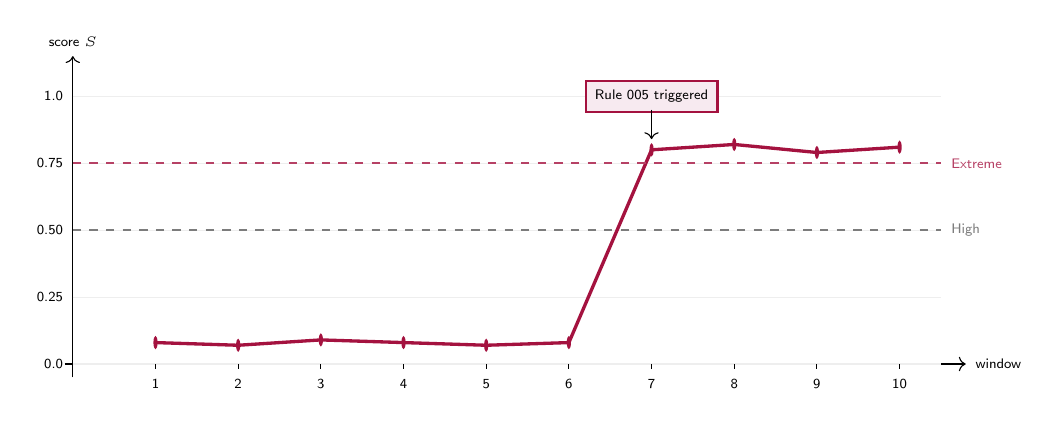
\begin{tikzpicture}[font=\tiny, xscale=1.05, yscale=3.4]
      % Axes
      \draw[->] (-0.1,0) -- (10.8,0) node[right] {window};
      \draw[->] (0,-0.05) -- (0,1.15) node[above] {score $S$};
      % Y grid + ticks
      \foreach \y in {0.0, 0.25, 0.50, 0.75, 1.0}{
        \draw[lightgray] (0,\y) -- (10.5,\y);
        \node[left] at (0,\y) {\y};
      }
      % X ticks
      \foreach \x in {1,...,10}{
        \draw (\x, 0) -- (\x, -0.02) node[below] {\x};
      }
      % Baseline phase (windows 1-6) flat ~0.08
      \draw[amritaMaroon, very thick]
        (1,0.08)--(2,0.07)--(3,0.09)--(4,0.08)--(5,0.07)--(6,0.08);
      % Anomaly jump windows 7-10
      \draw[amritaMaroon, very thick]
        (6,0.08)--(7,0.80)--(8,0.82)--(9,0.79)--(10,0.81);
      % Thresholds
      \draw[dashed, darkgray!70, thick] (0,0.50) -- (10.5,0.50)
            node[right, font=\tiny] {High};
      \draw[dashed, amritaMaroon!80, thick] (0,0.75) -- (10.5,0.75)
            node[right, font=\tiny] {Extreme};
      % Anomaly annotation
      \node[fill=lightmaroon, draw=amritaMaroon, thick,
            align=center, font=\tiny] at (7,1.0)
            {Rule 005 triggered};
      \draw[->, thin] (7,0.95) -- (7,0.84);
      % Data points
      \foreach \x/\y in {1/0.08,2/0.07,3/0.09,4/0.08,5/0.07,6/0.08,
                          7/0.80,8/0.82,9/0.79,10/0.81}{
        \fill[amritaMaroon] (\x,\y) circle (0.025cm);
      }
    \end{tikzpicture}%
  }%
}\\[0.05cm]
{\scriptsize\textbf{Fig. 17(a):} Pilot-dataset context and behavioural-drift visualisation}
\end{minipage}}

\vspace{0.1cm}
\begin{block}{Pilot Dataset}
\scriptsize The public pilot release contains \textbf{216} controlled-trial metadata records across multiple workloads, scenarios, and runtime contexts. It supports provenance and experiment design.
\end{block}
\end{frame}

% ===========================================================
% SLIDE 20 — Prototype Demonstration
% ===========================================================
\begin{frame}{18. Prototype Demonstration (2/2)}
\framesubtitle{Working Prototype Snapshot: Live Telemetry \& Behavioural Monitoring}
\centering
\fbox{\begin{minipage}[c][4.4cm]{0.96\textwidth}
\centering
\IfFileExists{images/prototype_demo_snapshot.png}{%
  \includegraphics[width=\textwidth,height=3.85cm,keepaspectratio]{images/prototype_demo_snapshot.png}%
}{%
  \IfFileExists{prototype_demo_snapshot.png}{%
    \includegraphics[width=\textwidth,height=3.85cm,keepaspectratio]{prototype_demo_snapshot.png}%
  }{%
    \textbf{[Working Prototype / Operational Dashboard Screenshot]}\\[0.2cm]
    {\scriptsize\itshape prototype\_demo\_snapshot.png}\\[0.3cm]
    {\scriptsize Replace this placeholder with a screenshot of the Porygon dashboard\\
    showing live telemetry, incident list, and scoring output.}
  }%
}\\[0.05cm]
{\scriptsize\textbf{Fig. 17(b):} Porygon operational dashboard and runtime telemetry view}
\end{minipage}}

\vspace{0.1cm}
\begin{block}{Demonstration Overview}
\scriptsize Falco eBPF tracepoints supply process-execution telemetry for behavioural assessment. Porygon records the resulting score and matched rules, retains event evidence for review, and stages containment only after explicit operator approval. The dashboard presents findings, evidence chain, and approval controls.
\end{block}
\end{frame}

% ===========================================================
% SLIDE 21 — Recorded Verification Results
% ===========================================================
\begin{frame}{19. Recorded Verification Results}
\small
\begin{table}\centering
\begin{tabularx}{\textwidth}{X l}\toprule
\textbf{Claim} & \textbf{Status} \\\midrule
Event-to-finding path & Verified in recorded runtime exercises \\
Lifecycle ingestion & 131 identities reconciled across collection, API, persistence, replay \\
Replay safety & 0 duplicate rows after replay \\
Runtime evidence & 8 live attack/control cases met expected evidence checks \\
Telemetry probe records & 11 Falco probe records successfully ingested \\
Rule governance & Preview, shadow review, activation, rollback, disable paths completed \\
Containment & Approved pause and rollback completed on a disposable container \\
\bottomrule
\end{tabularx}
\end{table}
\begin{block}{Comparative Study}
The controlled profile-scope evaluation measures false alarms, scenario recall, and scoring coverage on the same workload runs.
\end{block}
\end{frame}

% ===========================================================
% SLIDE 22 — Comparative Evaluation Protocol
% ===========================================================
\begin{frame}{20. Comparative Baseline Evaluation Protocol}
\begin{enumerate}
  \item Use pinned OCI images representing different workload roles.
  \item Define benign and anomalous scenarios with explicit ground truth.
  \item Compare global, tag, digest, and digest-plus-context profiles using the same workload runs.
  \item Keep baseline-building, validation, and final-evaluation data disjoint.
  \item Freeze calibration before held-out evaluation; report results per workload run.
  \item Reconcile generated events with backend-persisted telemetry.
\end{enumerate}
\begin{block}{Study Outputs}
False alarms, scenario recall, insufficient-profile outcomes, scoring coverage, and capture reconciliation. Pilot dataset published on Kaggle under CC BY 4.0 (216 records).
\end{block}
\end{frame}

% ===========================================================
% SLIDE 23 — Performance and Overhead
% ===========================================================
\begin{frame}{21. Performance and Overhead}
\small

\begin{table}\centering
\renewcommand{\arraystretch}{1.4}
\begin{tabularx}{0.96\textwidth}{l X r}
\toprule
\textbf{Component} & \textbf{Metric} & \textbf{Observed Value} \\\midrule
Falco eBPF sensor       & CPU overhead (idle host)         & $<1\%$ \\
Telemetry adapter       & Event throughput (SQLite spool)   & $>500$ events/s \\
Backend scoring         & Latency per window ($<10$k events) & $<200$\,ms \\
PostgreSQL              & Storage per event (with JSON snapshot) & $\approx2$\,KB \\
Dashboard               & Load time (static assets)         & $<100$\,ms \\
\bottomrule
\end{tabularx}
\end{table}

\vspace{0.2cm}
\begin{alertblock}{Footnote}
Values observed on development hardware; \textbf{not} a production benchmark. No controlled throughput stress test has been conducted.
\end{alertblock}
\end{frame}

% ===========================================================
% SLIDE 24 — Technical Justification
% ===========================================================
\begin{frame}{22. Technical Justification and Trade-offs}
\begin{itemize}
  \item \textbf{Digest-scoped profiles:} Preserve workload context; avoid silently pooling different image contents.
  \item \textbf{Jensen--Shannon distance:} Bounded distributional comparison that remains finite for categories observed on only one side.
  \item \textbf{Hybrid method:} Scores summarise behavioural change; rules identify the evidence that produced a finding.
  \item \textbf{Approval gate:} Avoids disruptive automatic action based solely on an anomaly score.
  \item \textbf{Trade-off:} Monitoring process and lifecycle events does not capture every aspect of runtime behaviour (see Limitations).
\end{itemize}
\end{frame}

% ===========================================================
% SLIDE 25 — Limitations & Operational Boundaries
% ===========================================================
\begin{frame}{23. Limitations \& Operational Boundaries}
\begin{columns}[T,onlytextwidth]
\column{0.50\textwidth}
\begin{block}{What We Observe}
\centering
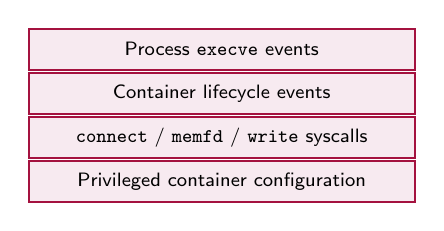
\begin{tikzpicture}[font=\scriptsize, node distance=0.18cm]
  \foreach \txt/\idx in {%
    {Process \texttt{execve} events}/0,
    {Container lifecycle events}/1,
    {\texttt{connect} / \texttt{memfd} / \texttt{write} syscalls}/2,
    {Privileged container configuration}/3%
  }{
    \node[draw=amritaMaroon, fill=lightmaroon, thick,
          minimum width=4.9cm, minimum height=0.52cm, align=center,
          yshift={-\idx*0.56cm}] (lo\idx) {\txt};
  }
\end{tikzpicture}
\end{block}

\column{0.47\textwidth}
\begin{alertblock}{What We Cannot Observe}
\centering
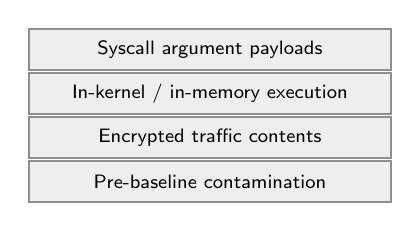
\begin{tikzpicture}[font=\scriptsize, node distance=0.18cm]
  \foreach \txt/\idx in {%
    {Syscall argument payloads}/0,
    {In-kernel / in-memory execution}/1,
    {Encrypted traffic contents}/2,
    {Pre-baseline contamination}/3%
  }{
    \node[draw=darkgray!60, fill=lightgray, thick,
          minimum width=4.6cm, minimum height=0.52cm, align=center,
          yshift={-\idx*0.56cm}] (ro\idx) {\txt};
  }
\end{tikzpicture}
\end{alertblock}
\end{columns}

\vspace{0.2cm}
\begin{itemize}\small
  \item Baseline contamination causes malicious activity to be learned as normal.
  \item Workload drift can change legitimate behaviour and raise false alarms.
  \item Pause and stop remain approval-gated because they affect workload availability.
\end{itemize}
\end{frame}

% ===========================================================
% SLIDE 26 — Future Work
% ===========================================================
\begin{frame}{24. Future Work \& Next Validation Stage}
\begin{itemize}
  \item Execute the comparative profile-scope evaluation across more images and workloads.
  \item Measure telemetry loss and workload overhead separately on representative hardware.
  \item Compare rules-only, distance-only, novelty-only, and combined scoring in isolation.
  \item Extend runtime evidence surface to include \texttt{connect} and \texttt{memfd\_create} syscall context.
  \item Investigate automated baseline refresh with explicit contamination safeguards.
  \item Publish full evaluation dataset with per-run provenance (CC BY 4.0).
\end{itemize}
\end{frame}

% ===========================================================
% SLIDE 27 — Research Contributions
% ===========================================================
\begin{frame}{25. Research Contributions}
\centering
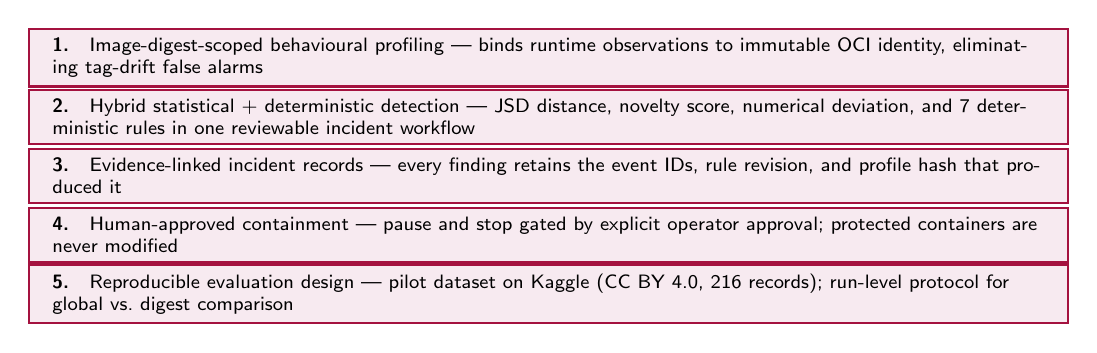
\begin{tikzpicture}[font=\scriptsize, node distance=0.22cm]

  \foreach \num/\txt/\idx in {%
    {1}/{Image-digest-scoped behavioural profiling — binds runtime observations to immutable OCI identity, eliminating tag-drift false alarms}/0,
    {2}/{Hybrid statistical + deterministic detection — JSD distance, novelty score, numerical deviation, and 7 deterministic rules in one reviewable incident workflow}/1,
    {3}/{Evidence-linked incident records — every finding retains the event IDs, rule revision, and profile hash that produced it}/2,
    {4}/{Human-approved containment — pause and stop gated by explicit operator approval; protected containers are never modified}/3,
    {5}/{Reproducible evaluation design — pilot dataset on Kaggle (CC BY 4.0, 216 records); run-level protocol for global vs.\ digest comparison}/4%
  }{
    \node[draw=amritaMaroon, fill=lightmaroon, thick,
          minimum width=13.0cm, minimum height=0.68cm, align=left,
          text width=12.6cm,
          inner xsep=0.3cm, yshift={-\idx*0.75cm}]
          {\textbf{\num.}\quad\txt};
  }

\end{tikzpicture}
\end{frame}

% ===========================================================
% SLIDE 28 — References
% ===========================================================
\begin{frame}[allowframebreaks]{References}
\footnotesize
\begin{thebibliography}{14}
\bibitem{oci} Open Container Initiative, ``OCI Image Format Specification.'' [Online]. Available: \url{https://github.com/opencontainers/image-spec}
\bibitem{abed} A. S. Abed, T. C. Clancy, and D. S. Levy, ``Applying bag of system calls for anomalous behavior detection of applications in Linux containers,'' in \textit{Proc. IEEE Globecom Workshops}, 2015.
\bibitem{castanhel} G. R. Castanhel, T. Heinrich, F. Ceschin, and C. A. Maziero, ``Taking a peek: An evaluation of anomaly detection using system calls for containers,'' in \textit{Proc. IEEE ISCC}, 2021, doi: 10.1109/ISCC53001.2021.9631251.
\bibitem{elkhairi} A. El Khairi et al., ``Contextualizing system calls in containers for anomaly-based intrusion detection,'' in \textit{Proc. Cloud Computing Security Workshop}, 2022, doi: 10.1145/3560810.3564266.
\bibitem{fournier} G. Fournier, S. Afchain, and S. Baubeau, ``Runtime security monitoring with eBPF,'' in \textit{Proc. SSTIC}, 2021.
\bibitem{falco} The Falco Authors, ``Falco: Cloud-native runtime security.'' [Online]. Available: \url{https://falco.org/}
\bibitem{lin} X. Lin et al., ``eBPF-Guard: A detection method for container escape via multi-level monitoring and enhanced analysis model,'' \textit{Empirical Software Engineering}, vol. 31, art. 51, 2026, doi: 10.1007/s10664-025-10784-1.
\bibitem{xiong} K. Xiong, Z. Wu, and X. Jia, ``DeepContainer: A deep learning-based framework for real-time anomaly detection in cloud-native container environments,'' \textit{J. Advanced Computing Systems}, vol. 5, no. 1, 2025, doi: 10.69987/JACS.2025.50101.
\bibitem{kim} J. Kim et al., ``Class label-aware graph anomaly detection,'' in \textit{Proc. ACM CIKM}, 2023. [Online]. Available: \url{https://arxiv.org/abs/2308.11669}
\bibitem{petrovic} I. Petrovic et al., ``Framework for semantic threat detection in Docker container environments with local MoE LLMs,'' \textit{Electronics}, vol. 15, no. 8, art. 1664, 2026, doi: 10.3390/electronics15081664.
\bibitem{bouke} M. A. Bouke et al., ``Multi-level distributional entropy for explainable network intrusion detection,'' arXiv:2606.29797, 2026.
\bibitem{linjs} J. Lin, ``Divergence measures based on the Shannon entropy,'' \textit{IEEE Trans. Information Theory}, vol. 37, no. 1, pp. 145--151, 1991, doi: 10.1109/18.61115.
\bibitem{endres} D. M. Endres and J. E. Schindelin, ``A new metric for probability distributions,'' \textit{IEEE Trans. Information Theory}, vol. 49, no. 7, pp. 1858--1860, 2003, doi: 10.1109/TIT.2003.813506.
\bibitem{hoyos} J. K. Hoyos-Osorio and L. G. Sanchez-Giraldo, ``The representation Jensen--Shannon divergence,'' \textit{NeurIPS}, 2023. [Online]. Available: \url{https://arxiv.org/abs/2305.16446}
\end{thebibliography}
\end{frame}

% ===========================================================
% SLIDE 29 — Thank You
% ===========================================================
\begin{frame}[plain]\centering\vfill
{\Huge\bfseries\color{amritaMaroon}Thank You}\\[0.35cm]
{\Large Questions \& Viva Voce}\vfill
\end{frame}

\end{document}
